%% %% %% %%
%%
%% Parte B de la práctica
%%
%% %% %% %%

\documentclass[../procedimientos.tex]{subfiles}
\graphicspath{{\subfix{../../images/}}}

\begin{document}
\subsection{Parte B}
\subsubsection{Instrucciones}
\begin{em}
  Construir de manera gráfica las siguientes compuertas lógicas y simularlas 
  dentro de la plataforma Quartus.
  \begin{itemize}
    \item NAND (y su forma expandida)
    \item NOR (y su forma expandida)
    \item XNOR (y su forma expandida)
  \end{itemize}
\end{em}

\subsubsection{Análisis}
De igual forma que en la sección anterior, es importante tener presente el 
comportamiento de cada una de las compuertas con la finalidad de comprobar de 
forma satisfactoria el resultado de la actividad. La tabla de verdad de cada 
una de las compuertas se muestra a continuación:
\begin{table}[h!]
  \caption{Tablas de verdad (Sección B)}
  \label{tab:b_tv}
  \centering
  \begin{subtable}[t]{0.25\linewidth} % Compuerta AND
    \centering
    \label{tab:comp_nand}
    \begin{tabular}{|c c|c|}
      \hline
      $A$ & $B$ & $\overline{A \cdot B}$\\
      \hline
      0 & 0 & 1\\
      0 & 1 & 1\\
      1 & 0 & 1\\
      1 & 1 & 0\\
      \hline
    \end{tabular}
    \caption{Compuerta NAND}
  \end{subtable}
  \begin{subtable}[t]{0.25\linewidth} % Compuerta OR
    \centering
    \label{tab:comp_nor}
    \begin{tabular}{|c c|c|}
      \hline
      $A$ & $B$ & $\overline{A + B}$\\
      \hline
      0 & 0 & 1\\
      0 & 1 & 0\\
      1 & 0 & 0\\
      1 & 1 & 0\\
      \hline
    \end{tabular}
    \caption{Compuerta NOR}
  \end{subtable}
  \begin{subtable}[t]{0.25\linewidth} % Compuerta XOR
    \centering
    \label{tab:comp_xnor}
    \begin{tabular}{|c c|c|}
      \hline
      $A$ & $B$ & $\overline{A \oplus B}$\\
      \hline
      0 & 0 & 1\\
      0 & 1 & 0\\
      1 & 0 & 0\\
      1 & 1 & 1\\
      \hline
    \end{tabular}
    \caption{Compuerta XNOR}
  \end{subtable}
\end{table}

Todas las compuertas anteriores tienen una equivalencia usando úncamente las 
compuertas AND, OR y NOT, tal como se muestra a continuación.
\begin{align}
  \overline{A \cdot B} &= \nt{A} + \nt{B}\\
  \overline{A + B} &= \nt{A} \cdot \nt{B}\\
  \overline{A \oplus B} &= \nt{A} \cdot \nt{B} + A \cdot B
\end{align}

\subsubsection{Desarrollo en Quartus}
Se comenzó esta actividad partiendo de lo que ya se había hecho anteriormente 
en la actividad A. El diagrama del sistema quedó de la siguiente forma:
\begin{figure}[H]
  \centering
  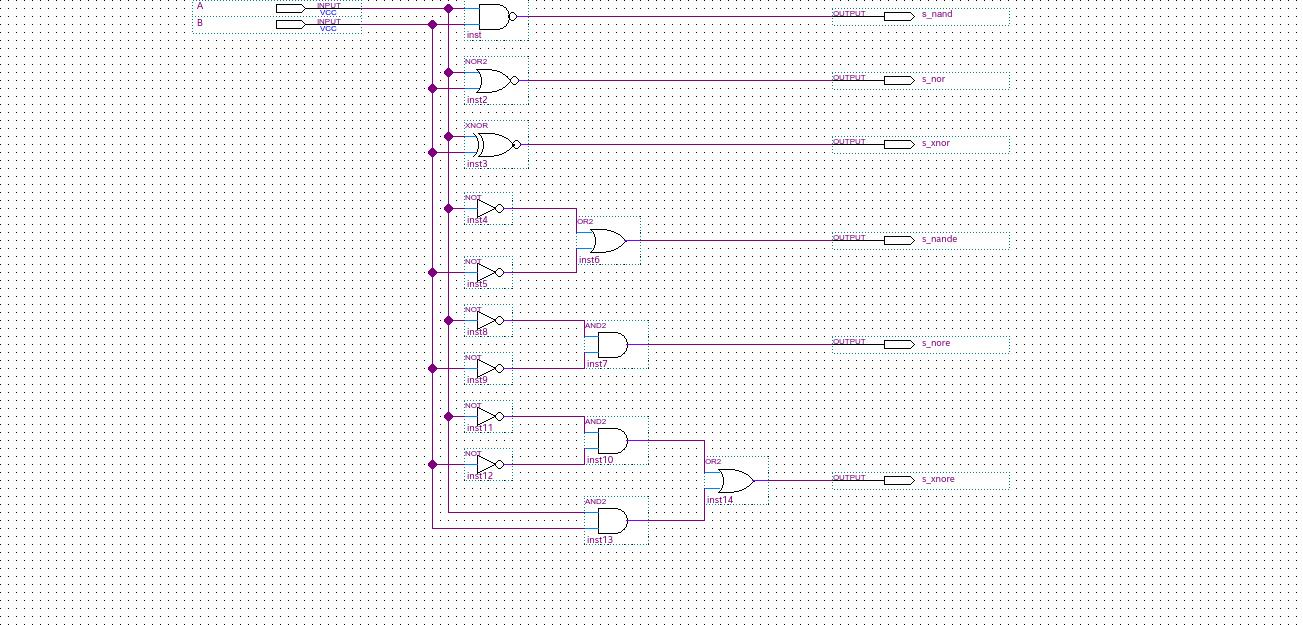
\includegraphics[width=0.9\textwidth]{inciso_b_schematic}
  \caption{Esquema del funcionamiento de las seis compuertas (Sección B)}
\end{figure}

Posteriormente, se creó otro archivo con formato \textit{University Program 
VWF}, a través del cual se pudo realizar un \textbf{cronograma} con las 
señales de entrada y salida de simulación. La configuración de las señales de 
entrada se muestra a continuación:
\begin{figure}[H]
  \centering
  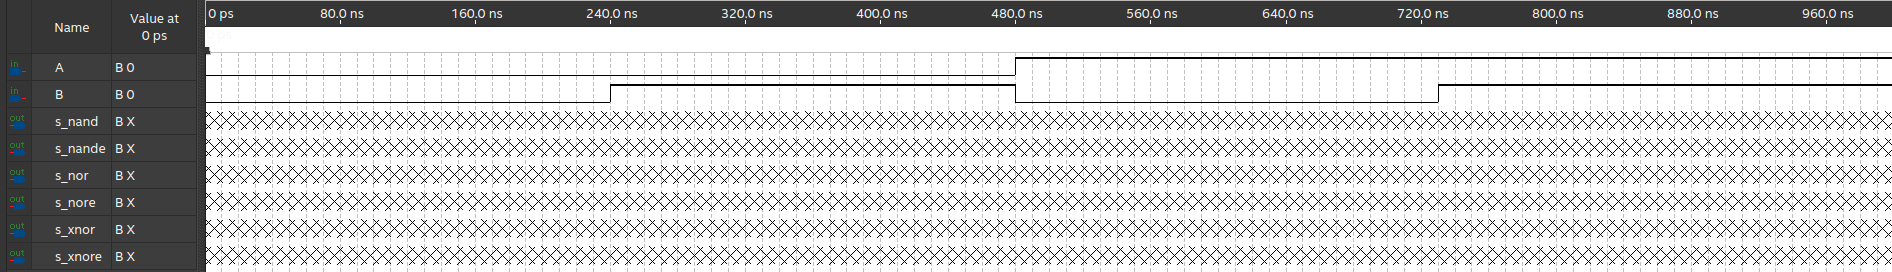
\includegraphics[width=\textwidth]{inciso_b_cron_1}
  \caption{Alternación de los valores de $A$ y $B$ (Sección B)}
  \label{fig:variables_cron_b}
\end{figure}

Tal como se puede apreciar, se tienen las siguientes señales. Por un lado 
están las entradas:
\begin{itemize}
  \item $A$
  \item $B$
\end{itemize}

y por otro lado se tienen las salidas:
\begin{itemize}
  \item $s\_nand$: La salida de la compuerta NAND.
  \item $s\_nor$: La salida de la compuerta NOR.
  \item $s\_xnor$: La salida de la compuerta XNOR.
  \item $s\_nande$: La salida de la compuerta NAND equivalente.
  \item $s\_nore$: La salida de la compuerta NOR equivalente.
  \item $s\_xnore$: La salida de la compuerta XNOR equivalente.
\end{itemize}


Al ejecutar la \textit{Simulación Funcional} se obtuvo lo siguiente:
\begin{figure}[H]
  \centering
  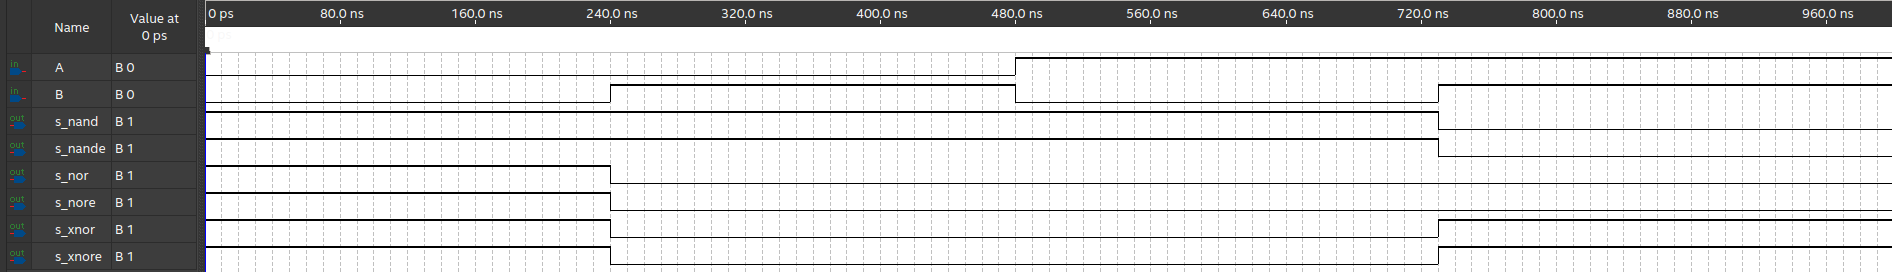
\includegraphics[width=\textwidth]{inciso_b_cron_2}
  \caption{Cronograma del sistema (Sección B)}
  \label{fig:cron_b}
\end{figure}

En la parte anterior, se pueden verificar dos cosas:
\begin{enumerate}
  \item Que las compuertas extendidas tienen el mismo comportamiento que sus 
    compuertas correspondientes.
  \item Que el comportamiento de las compuertas en la Figura \ref{fig:cron_b} 
    es el mismo que el descrito por las tablas de verdad de la Tabla 
    \ref{tab:b_tv}.
\end{enumerate}

\end{document}


